\documentclass{article}

\usepackage{etoolbox}
\newtoggle{arxiv}
% \togglefalse{arxiv}
\toggletrue{arxiv}

\usepackage[utf8]{inputenc} % allow utf-8 input
\usepackage[T1]{fontenc}    % use 8-bit T1 fonts
\usepackage{hyperref}       % hyperlinks
\usepackage{url}            % simple URL typesetting
\usepackage{booktabs}       % professional-quality tables
\usepackage{amsfonts}       % blackboard math symbols
\usepackage{nicefrac}       % compact symbols for 1/2, etc.
\usepackage{microtype}      % microtypography
\usepackage{xcolor}         % colors
\usepackage{amsmath,amsthm,amssymb}

\usepackage{algorithm}
\usepackage{algorithmic}

\usepackage{subcaption}
\usepackage{multirow}

\usepackage{xspace}
\usepackage{wrapfig}

% the X mark
\usepackage{pifont}
\newcommand{\xmark}{\ding{55}}

\usepackage[capitalise]{cleveref}  % Otherwise I get an error saying cleveref must be loaded after hyperref
\usepackage{comment}
\usepackage[inline]{enumitem}

\usepackage{graphicx}
\usepackage{grffile}
\usepackage{color}

% https://tex.stackexchange.com/questions/26637/how-do-you-get-mathbb1-to-work-characteristic-function-of-a-set
\usepackage{newtxmath}

\iftoggle{arxiv}{
\usepackage[numbers,sort]{natbib}
}{}

\usepackage{import}
% https://tex.stackexchange.com/questions/153312/subfiles-inside-a-subfile-using-relative-paths
\providecommand{\main}{.}

\newtoggle{todo}
\toggletrue{todo}
% \togglefalse{todo} % comment this line to show comments
\newcommand{\todo}[1]{\iftoggle{todo}{\textcolor{cyan}{[TODO: #1]}}{}}

\newtoggle{comment}
% \toggletrue{comment}
\togglefalse{comment} % comment this line to show comments
\newcommand{\TD}[1]{\iftoggle{comment}{\textcolor{magenta}{[TD: #1]}}{}}

\newcommand{\abs}[1]{\left\lvert#1\right\rvert}
\newcommand{\norm}[1]{\left\|{#1}\right\|} % A norm with 1 argument
\newcommand{\diag}{\mathrm{diag}}
\newcommand{\softmax}{\mathrm{softmax}}
\newcommand{\dsoftmax}{\mathrm{dsoftmax}}
\providecommand{\tr}{\mathop{\rm tr}}

\newcommand{\defeq}{:=}

\newcommand{\vQ}{\mathbf{Q}}
\newcommand{\vK}{\mathbf{K}}
\newcommand{\vV}{\mathbf{V}}
\newcommand{\vdQ}{\mathbf{dQ}}
\newcommand{\vdK}{\mathbf{dK}}
\newcommand{\vdV}{\mathbf{dV}}
\newcommand{\vS}{\mathbf{S}}
\newcommand{\vdS}{\mathbf{dS}}
\newcommand{\vP}{\mathbf{P}}
\newcommand{\vdP}{\mathbf{dP}}
\newcommand{\vU}{\mathbf{U}}
\newcommand{\vW}{\mathbf{W}}
\newcommand{\vT}{\mathbf{T}}
\newcommand{\vX}{\mathbf{X}}
\newcommand{\vO}{\mathbf{O}}
\newcommand{\vdO}{\mathbf{dO}}
\newcommand{\vM}{\mathbf{M}}
\newcommand{\vZ}{\mathbf{Z}}

\newcommand{\sysnameone}{\textsc{FlashAttention}\xspace}
\newcommand{\sysname}{\textsc{FlashAttention-2}\xspace}


\newtheorem{theorem}{Theorem}
\newtheorem*{theorem*}{Theorem}
\newtheorem{corollary}[theorem]{Corollary}
\newtheorem{definition}{Definition}
\newtheorem{lemma}[theorem]{Lemma}
\newtheorem{claim}[theorem]{claim}
\newtheorem{example}{Example}
\newtheorem{proposition}[theorem]{Proposition}

\iftoggle{arxiv}{
  \setlength{\textwidth}{6.5in}
  \setlength{\textheight}{9in}
  \setlength{\oddsidemargin}{0in}
  \setlength{\evensidemargin}{0in}
  \setlength{\topmargin}{-0.5in}
  \newlength{\defbaselineskip}
  \setlength{\defbaselineskip}{\baselineskip}
  \setlength{\marginparwidth}{0.8in}
}{
% --------------------
% Space-saving options
% comment now for longer appendix
\usepackage[compact]{titlesec}
\titlespacing{\section}{0pt}{*1}{*0}
\titlespacing{\subsection}{0pt}{*1.5}{*0}

\usepackage[subtle, mathdisplays=tight, charwidths=tight, leading=normal]{savetrees}
% \usepackage[subtle, mathdisplays=tight, charwidths=normal, leading=normal]{savetrees}
% \usepackage[subtle]{savetrees}

% Can always cheat a bit on the margins
% \addtolength\titlebox{-0.3in}
% \addtolength\columnsep{-0.15in}
% \addtolength\textwidth{0.15in}
% \addtolength\textheight{0.15in}
\addtolength\textfloatsep{-0.5em}
\addtolength\intextsep{-0.2em}

% https://tex.stackexchange.com/questions/146890/how-to-apply-looseness-1-to-all-the-paragraphs
% Does savetrees do this already?
% \linepenalty=1000

\def\setstretch#1{\renewcommand{\baselinestretch}{#1}}
\setstretch{0.985}
\addtolength{\parskip}{-1pt}

}

\title{\sysname:\\Faster Attention with Better Parallelism and Work Partitioning}

\iftoggle{arxiv}{
  \usepackage{authblk}
  \author[1,2]{Tri Dao}
  \affil[1]{Department of Computer Science, Princeton University}
  \affil[2]{Department of Computer Science, Stanford University}
  \affil[ ]{\texttt{trid@cs.stanford.edu}}
}{
}

\begin{document}


\maketitle


\begin{abstract}

\begin{abstract}
Language models (LMs), like other neural networks, often favor shortcut heuristics based on surface-level patterns.
Although LMs behave like n-gram models early in training, they must eventually learn hierarchical syntactic representations to correctly apply grammatical rules out-of-distribution (OOD).
In this work, we use case studies of English grammar to explore how complex, diverse training data drives models to generalize OOD. We construct a framework that unifies our understanding of random variation with training dynamics, rule selection with memorization, and data diversity with complexity. 
We show that these factors are nuanced, and that intermediate levels of diversity and complexity lead to inconsistent behavior across random seeds and to unstable training dynamics. 
Our findings emphasize the critical role of training data in shaping generalization patterns and illuminate how competing model strategies lead to inconsistent generalization outcomes across random seeds. Code is available at \url{https://github.com/sunnytqin/concept_comp.git}.

\end{abstract}

\end{abstract}

\section{Introduction}
%
Neural network (NN) learning has underpinned state of the art empirical
results in numerous applied machine learning tasks (see for
instance~\cite{krizhevsky2012imagenet,lecun2015deep}). Nonetheless, neural
network learning remains rather poorly understood in several regards.
Notably, it remains unclear why training algorithms find good weights, how
learning is impacted by the network architecture and activations, what is
the role of random weight initialization, and how to choose a concrete
optimization procedure for a given architecture.

We start by analyzing the expressive power of NNs subsequent to the random
weight initialization. The motivation is the empirical success of training
algorithms despite inherent computational intractability, and the fact that
they optimize highly non-convex objectives with potentially many local minima.
Our key result shows that random initialization already positions learning
algorithms at a good starting point. We define an object termed a {\em
computation skeleton} that describes a distilled structure of feed-forward
networks. A skeleton induces a family of network architectures along with a
hypothesis class $\ch$ of functions obtained by certain non-linear
compositions according to the skeleton's structure.  We show that the
representation generated by random initialization is sufficiently rich to
approximately express the functions in $\ch$. Concretely, all functions in
$\ch$ can be approximated by tuning the weights of the last layer, which is
a convex optimization task.

In addition to explaining in part the success in finding good weights, our
study provides an appealing perspective on neural network learning.  We
establish a tight connection between network architectures and their dual
kernel spaces. This connection generalizes several previous constructions
(see Sec~\ref{sec:related}). As we demonstrate, our dual view gives rise to
design principles for NNs, supporting current practice and suggesting
new ideas. We outline below a few points.

\begin{itemize}

\item Duals of convolutional networks appear a more suitable fit for
	vision and acoustic tasks than those of fully connected networks.

\item Our framework surfaces a principled initialization scheme. It is
	very similar to common practice, but incorporates a small correction.

\item By modifying the activation functions, two consecutive fully connected
	layers can be replaced with one while preserving the network's dual kernel.

\item The ReLU activation, i.e. $x \mapsto \max(x,0)$, possesses favorable
	properties. Its dual kernel is expressive, and it can be well approximated by
	random initialization, even when the initialization's scale is moderately
	changed.

\item As the number of layers in a fully connected network becomes very
	large, its dual kernel converges to a degenerate form for any non-linear
	activation.

\item Our result suggests that optimizing the weights of the last layer can
	serve as a convex proxy for choosing among different architectures prior
	to training. This idea was advocated and tested empirically
	in~\cite{saxe2011random}.

\end{itemize}



\section{Experimental Setup}
\label{sec:experiments}
The question formation task and the tense inflection task were first proposed by \citet{Frank2007-pn} and \citet{Linzen2016-vx} as canonical tests of language modeling ability. We use existing synthetic datasets for question formation from \citet{McCoy2018-uv} and tense inflection from \citet{McCoy2020-pj}.
\subsection{Question Formation Task}
\label{sec:qf_task}
\begin{table}[t]
    \centering
    {\renewcommand{\arraystretch}{1.12}
    \small
      \caption{\textbf{Examples from two grammar case studies.} \textit{Top}: In the question formation task, the model moves the main auxiliary verb to the front to form a question.
      \textit{Bottom}:  In the tense inflection task, the model inflects the main verb from past to present tense, while respecting subject-verb agreement. }  
    \label{tab:task_examples}
    \resizebox{\textwidth}{!}{
    \begin{tabular}{p{2.5cm} p{2.3cm} p{9cm}}
    \toprule
    \textbf{Dataset} & \textbf{Task Type} & \hspace{3.5cm} \textbf{Examples} \\ 
    \hline
    \multirow{2}{*}{Question Formation} & Quest  & \textbf{Input:} My unicorn \textcolor{ForestGreen}{does} move the dogs that \textcolor{red}{do} wait.  \\ 
                             &(Ambiguous)  &\textbf{Output:} \textcolor{ForestGreen}{Does} my unicorn move the dogs that \textcolor{red}{do} wait?     \\
                             \cline{2-3} 
                             & \multirow{2}{*}{Quest }   &\textbf{Input:} My unicorn who \textcolor{red}{doesn't} sing \textcolor{ForestGreen}{does} move.
 \\ 
                             & & \textbf{Linear Output:} \textcolor{red}{Doesn't} my unicorn who sing \textcolor{ForestGreen}{does} move?
 \\
                             & (Unambiguous)& \textbf{Hierarchical Output:} \textcolor{ForestGreen}{Does} my unicorn who \textcolor{red}{doesn't} sing move? \\
                              
                             % & \multirow{2}{*}{Decl}   & \textbf{Input:} My unicorn does move the dogs that do wait. \\ 
                             % & & \textbf{Output:} My unicorn does move the dogs that do wait.    \\
    \hline
    \multirow{5}{*}{Tense Inflection} & Present & \textbf{Input:} My zebra behind the peacock smiled. \\ 
                        & (Ambiguous) & \textbf{Output:} My \textcolor{cyan}{zebra} behind the \textcolor{cyan}{peacock}  \textcolor{ForestGreen}{smiles}.    \\
                        \cline{2-3} 
                        & \multirow{1.5}{*}{Present}   & \textbf{Input:} My zebra behind the peacocks smiled. \\ 
                        & & \textbf{Linear output:} My zebra behind the \textcolor{cyan}{peacocks} \textcolor{red}{smile}.     \\
                        &  (Unambiguous) & \textbf{Hierarchical output:} My \textcolor{red}{zebra} behind the peacocks \textcolor{ForestGreen}{smiles}.     \\
                        % & \multirow{2}{*}{Decl}   & Input: My unicorn does move the dogs that do wait. \\ 
                        % & & Output: My unicorn does move the dogs that do wait.    \\
    \bottomrule
    \end{tabular}
    \vspace{-5px}
    }}
\end{table}


In the \textbf{question formation (QF)} task, the model transforms a declarative sentence into a question (see Table~\ref{tab:task_examples}) by moving the main auxiliary verb (such as \textit{does} in \textit{does move}) to the front. Our training data (based on \citet{McCoy2018-uv}) permits two strategies for choosing which verb to move: (1) a linear rule that moves the first auxiliary verb (Figure \ref{fig:stability_demo} \textit{upper right}), or (2) a hierarchical rule---the correct rule in English grammar---based on the sentence's syntax tree (Figure \ref{fig:stability_demo} \textit{lower right}). The model leverages this tree representation to select the main auxiliary verb.

Examples of each rule are provided in Table \ref{tab:task_examples}. The first example is considered \textbf{ambiguous} because the hierarchical and linear rules produce the same correct outcome. In contrast, the second example is \textbf{unambiguous} because only the hierarchical rule produces the correct outcome. The training and in-distribution test data contain only ambiguous samples, while the OOD generalization set includes only unambiguous samples. Therefore, if a model uses the hierarchical rule, it will achieve $100\%$ accuracy on both the in-distribution (ambiguous questions) and OOD (unambiguous questions) sets. Conversely, if a model uses the linear rule, it will still achieve 100\% accuracy on the in-distribution set, but will score $0\%$ on the OOD set. 
We therefore use the model's accuracy on the OOD set to measure hierarchical generalization.


\subsection{Tense Inflection Task}
\label{sec:ti_task}

In the \textbf{tense inflection (TI)} task, the model transforms a past-tense sentence into the present tense by changing the inflection of its main verb. 
Since past-tense verbs in English have the same form in singular and plural, the model must identify the subject to determine whether the present-tense verb should be inflected as singular or plural. The TI model could follow either a hierarchical or linear rule for subject-verb agreement in the training data (based on \citet{McCoy2020-pj}). The linear rule inflects the verb based on the most recent noun, while the hierarchical rule correctly inflects the verb according to its subject. As in the QF task, the training and in-distribution test sets contain ambiguous examples, whereas the OOD set contains unambiguous examples. In the ambiguous example from Table \ref{tab:task_examples}, the subject noun \textit{zebra} and the most recent noun \textit{peacock} must share the same plurality and therefore either rule produces the correct answer. In the OOD unambiguous example, the subject and the most recent noun differ in plurality and therefore only the hierarchical rule produces the correct answer.
Similar to the QF task, we use the model's main-verb prediction accuracy on the OOD set as a metric for hierarchical generalization.


\subsection{Models, Data and Training}
\label{sec:model_and_training}
We run all experiments on the same 50 random seeds using hyperparameter settings from the existing literature \citep{Ahuja2024-ul, Murty2023-xp}. We use a decoder-only Transformer architecture where each layer has 8 heads with a 512-dimensional embedding. QF models have 6 layers and TI models have 4 layers. All models are trained from scratch on a causal language modeling objective for 300K steps. We use the Adam optimizer \citep{Kingma2014-he}, a learning rate of 1e-4, and a linear decay schedule. We use a word-level tokenizer with a vocabulary of size 72. 

We use the original training, validation and OOD generalization data proposed by \citet{McCoy2018-uv} and \citet{McCoy2020-pj}. To create variations on the training data, we mimic the data generation process used for the original QF and TI task. Specifically, the original TI and QF data are generated with Context-Free Grammars (CFGs) using a simplified set of grammatical rules; we reuse the same CFG rules to create variations of the training data. 



\section{FlashAttention-3: Algorithm}
\label{sec:algo}

In this section, we describe the \fat algorithm. For simplicity, we focus on the
forward pass, with the backward pass algorithm described in~\cref{sec:algo_ws_bwd}. We first indicate how to integrate warp-specialization with a circular SMEM buffer into the base algorithm of \faa. We then explain how to exploit asynchrony of WGMMA to define an overlapped GEMM-softmax 2-stage pipeline. Finally, we describe the modifications needed for FP8, both in terms of layout conformance and accuracy via block quantization and incoherent processing.

\subsection{Producer-Consumer asynchrony through warp-specialization and
  pingpong scheduling}
\label{sec:algo_ws}

\paragraph{Warp-specialization}
As with \faa, the forward pass of \fat is embarrassingly parallel in the batch size, number of heads, and query sequence length.
Thus, it will suffice to give a CTA-level view of the algorithm, which operates on a tile $\vQ_i$ of the query matrix to compute the corresponding tile $\vO_i$ of the output.
To simplify the description, we first give the warp-specialization scheme with a circular SMEM buffer that does \emph{not} have in addition the GEMM-softmax overlapping.
Let $d$ be the head dimension, $N$ the sequence length, and fix a query block size $B_r$ to divide $\vQ$ into $T_r = \lceil \frac{N}{B_r} \rceil$ blocks $\vQ_1, .., \vQ_{T_r}$.

\begin{algorithm}[H]
    \caption{\small\label{alg:flash3_wgmma_ws_only}\fat forward pass \textbf{without} intra-consumer overlapping -- CTA view}
    \begin{algorithmic}[1]
\REQUIRE Matrices $\vQ_i \in \RR^{B_r \times d}$ and $\vK, \vV \in \mathbb{R}^{N \times d}$ in HBM, key block size $B_c$ with $T_c = \lceil \frac{N}{B_c} \rceil$.
\STATE Initialize pipeline object to manage barrier synchronization with $s$-stage circular SMEM buffer.
\IF {in producer warpgroup}
\STATE Deallocate predetermined number of registers.
\STATE Issue load $\vQ_i$ from HBM to shared memory.
\STATE Upon completion, commit to notify consumer of the load of $\vQ_i$.
\FOR{$0 \le j < T_c$}
    \STATE Wait for the $(j\,\%\,s)$th stage of the buffer to be consumed.
    \STATE Issue loads of $\vK_j, \vV_j$ from HBM to shared memory at the $(j\,\%\,s)$th stage of the buffer.
    \STATE Upon completion, commit to notify consumers of the loads of $\vK_j, \vV_j$.
\ENDFOR
\ELSE
\STATE Reallocate predetermined number of registers as function of number of consumer warps.
\STATE On-chip, initialize $\vO_i = (0) \in \mathbb{R}^{B_r \times d}$ and $\ell_i, m_i = (0), (-\infty) \in \mathbb{R}^{B_r}$.
\STATE Wait for $\vQ_i$ to be loaded in shared memory.
\FOR{$0 \le j < T_c$}
\STATE Wait for $\vK_j$ to be loaded in shared memory.
\STATE Compute $\vS_i^{(j)} = \vQ_i \vK_j^T$ (SS-GEMM). Commit and wait. \label{alg:ws_only_gemm1}
\STATE Store $m_i^{\mathrm{old}} = m_i$ and compute $m_i = \max(m_i^{\mathrm{old}}, \rowmax(\vS_i^{(j)}))$. \label{code-ws:softmax_start}
\STATE Compute $\widetilde{\vP}_i^{(j)} = \exp(\vS_i^{(j)} - m_i)$ and $\ell_i = \exp(m_i^{\mathrm{old}} - m_i) \ell_i + \rowsum(\widetilde{\vP}_i^{(j)})$. \label{code-ws:softmax_end}
\STATE Wait for $\vV_j$ to be loaded in shared memory.
\STATE Compute $\vO_i = \diag(\exp(m_i^{\mathrm{old}} - m_i))^{-1} \vO_i + \widetilde{\vP}_i^{(j)} \vV_j$ (RS-GEMM). Commit and wait. \label{alg:ws_only_gemm2}
\STATE Release the $(j\,\%\,s)$th stage of the buffer for the producer.
\ENDFOR
\STATE Compute $\vO_i = \diag(\ell_i)^{-1} \vO_i$ and $L_i = m_i + \log(\ell_i)$.
\STATE Write $\vO_i$ and $L_i$ to HBM as the $i$th block of $\vO$ and $L$.
\ENDIF
\end{algorithmic}
\end{algorithm}

For our implementation of \cref{alg:flash3_wgmma_ws_only} on Hopper, we use \verb|setmaxnreg| for (de)allocations, TMA for loads of $\vQ_i$ and $\{ \vK_j, \vV_j \}_{0 \leq j < T_c}$, and WGMMA to execute the GEMMs in the consumer mainloop, with the SS or RS prefix indicating whether the first operand is sourced from shared memory or register file.
For interpreting the execution flow of \cref{alg:flash3_wgmma_ws_only}, note that issuing TMA loads does not stall on the completion of other loads due to asynchrony.
Moreover, in the producer mainloop, no waits will be issued for the first $s$ iterations as the buffer gets filled.

\paragraph{Pingpong scheduling}
The asynchronous nature of WGMMA and TMA, along with warp-specialization, opens
up the opportunity to overlap the softmax computation of one warpgroup with the GEMM of
another warpgroup.
To motivate this, notice that non-matmul operations have much lower throughput
than matmul operations on modern hardware accelerators.
As an example, the H100 SXM5 GPU has 989 TFLOPS of FP16 matmul but only 3.9
TFLOPS of special functions such as exponential\footnote{The CUDA programming
  guide specifies that 16 operations of special functions can be performed per
  streaming multiprocessor (SM) per clock cycle. We multiply 16 by 132 SMs and
  1830 MHz clock speed to get 3.9 TFLOPS of special functions.} (necessary for softmax).
For the attention forward pass in FP16 with head dimension 128, there are 512x more matmul FLOPS
compared to exponential operations, but the exponential has 256x lower
throughput, so exponential can take 50\% of the cycle compared to matmul.
The situation is even worse with FP8, where the matmul throughput doubles but
the exponential throughput stays the same.

Since the exponential is performed by a separate hardware unit (the multi-function
unit), ideally we'd want the exponential calculation to be scheduled when the
Tensor Cores are performing the matmul.
To do so, we use synchronization barriers (\texttt{bar.sync} instructions) to
force the GEMMs (GEMM1 -- $\vP \vV$ of one iteration, and GEMM0 -- $\vQ \vK^\top$
of the next iteration) of warpgroup 1 to be scheduled before the GEMMs of
warpgroup 2.
As a result, the softmax of warpgroup 1 will be scheduled while warpgroup 2 is
performing its GEMMs. Then the roles swap, with warpgroup 2 doing softmax while
warpgroup 1 doing GEMMs (hence, ``pingpong'' scheduling).
This is illustrated in~\cref{fig:pingpong_scheduling}.
Though in practice the pingpong scheduling is not as clean as depicted in the
figure, we generally find this to improve performance (e.g., from 570 TFLOPS to
620-640 TFLOPS for FP16 forward with head dimension 128 and sequence length 8192).
\begin{figure}[ht]
    \centering
    \includegraphics[width=1.0\linewidth]{figs/pingpong_pipelining.png}
    \caption{Pingpong scheduling for 2 warpgroups to overlap softmax and GEMMs: the softmax of one warpgroup
      should be scheduled when the GEMMs of another warpgroup are running. The
      same color denotes the same iteration.}
    \label{fig:pingpong_scheduling}
\end{figure}

\paragraph{Attention variants}
For multi-query attention~\citep{shazeer2019fast} and grouped query
attention~\citep{ainslie2023gqa}, we follow the approach in \faa and adjust the
tensor indexing to avoid duplicating $\vK$ and $\vV$ in HBM.

\subsection{Intra-warpgroup overlapping GEMMs and softmax}


Even within one warpgroup, we can overlap some instructions in the softmax with
some instructions in the GEMMs. We describe one technique to do so.

In the attention algorithm, operations within the inner loop (main loop) have sequential dependencies that impede parallelization within a single iteration.
For example, (local) softmax (lines \ref{code-ws:softmax_start} to \ref{code-ws:softmax_end}) relies on the output $\vS_i^{(j)}$ of the first GEMM, while the second GEMM takes its result $\widetilde{\vP}_i^{(j)}$ as an operand.
Indeed, the wait statements in lines \ref{alg:ws_only_gemm1} and \ref{alg:ws_only_gemm2} of \cref{alg:flash3_wgmma_ws_only} serialize the execution of softmax and GEMMs.
However, we can break these dependencies by pipelining across iterations through additional buffers in registers.
Pursuing this idea, we propose the following two-stage\footnote{Note that the number of stages of the overlapping scheme is bounded by, but need not equal, the number $s$ of stages in the circular SMEM buffer.} GEMM-softmax pipelining algorithm:

\begin{figure}[ht]
    \centering
    \includegraphics[width=.95\linewidth]{figs/2_stage_pipelining.png}
    \caption{2-stage WGMMA-softmax pipelining}
    \label{fig:2_stage_pipelining}
\end{figure}

\begin{algorithm}[H]
    \caption{\small\label{alg:flash3_wgmma}\fat consumer warpgroup forward pass}
    \begin{algorithmic}[1]
      \REQUIRE  Matrices $\vQ_i \in \RR^{B_r \times d}$ and $\vK, \vV \in \mathbb{R}^{N \times d}$ in HBM, key block size $B_c$ with $T_c = \lceil \frac{N}{B_c} \rceil$.
      \STATE Reallocate predetermined number of registers as function of number of consumer warps.
      \STATE On-chip, initialize $\vO_i = (0) \in \mathbb{R}^{B_r \times d}$ and $\ell_i, m_i = (0), (-\infty) \in \mathbb{R}^{B_r}$.
      \STATE Wait for $\vQ_i$ and $\vK_0$ to be loaded in shared memory.
      \STATE Compute $\vS_{\mathrm{cur}} = \vQ_i \vK_0^T$ using WGMMA. Commit and wait.
      \STATE Release the $0$th stage of the buffer for $\vK$.
      \STATE Compute $m_{i}$, $\tilde{\vP}_{\mathrm{cur}}$ and $\ell_{i}$ based on $\vS_{\mathrm{cur}}$, and rescale $\vO_i$.
      \FOR{$1 \le j < T_c - 1$}
        \STATE Wait for $\vK_j$ to be loaded in shared memory.
        \label{code:mainloop_start}
        \STATE Compute $\vS_{\mathrm{next}} = \vQ_i \vK_{j}^T$ using WGMMA. Commit but do not wait. \label{code:first_wgmma}
        \STATE Wait for $\vV_{j-1}$ to be loaded in shared memory.
        \STATE Compute $\vO_{i} = \vO_{i} + \tilde{\vP}_{\mathrm{cur}} \vV_{j-1}$ using WGMMA. Commit but do not wait. \label{code:second_wgmma}
        \STATE Wait for the WGMMA $\vQ_i \vK_{j}^T$.
        \STATE Compute $m_{i}$, $\tilde{\vP}_{\mathrm{next}}$ and $\ell_{i}$ based on $\vS_{\mathrm{next}}$. \label{code:softmax}
        \STATE Wait for the WGMMA $\tilde{\vP}_{\mathrm{cur}} \vV_{j-1}$ and then rescale $\vO_i$
        \STATE Release the $(j\,\%\,s)$th, resp. $(j-1\,\%\,s)$th stage of the buffer for $\vK$, resp. $\vV$.
        \STATE Copy $\vS_{\mathrm{next}}$ to $\vS_{\mathrm{cur}}$.
        \label{code:mainloop_end}
      \ENDFOR
      \STATE Wait for $\vV_{T_c - 1}$ to be loaded in shared memory.
      \STATE Compute
      $\vO_{i} = \vO_{i} + \tilde{\vP}_{\mathrm{last}} \vV_{T_c - 1}$ using WGMMA. Commit and wait.

      \STATE Epilogue:
      Rescale $\vO_{i}$ based on $m_{i}$.
      Compute $L_{i}$ based on $m_{i}$ and $\ell_{i}$.
      Write $\vO_{i}$ and $L_{i}$ to HBM as the $i$-th block of $\vO$ and $L$.
    \end{algorithmic}
  \end{algorithm}

  \cref{alg:flash3_wgmma} functions as a replacement for the consumer path of \cref{alg:flash3_wgmma_ws_only} to comprise the complete \fat algorithm for FP16 precision. At a high-level, we use WGMMA as a metonym for asynchronous GEMM. Within the mainloop (lines \ref{code:mainloop_start} to \ref{code:mainloop_end}), the second WGMMA operation of iteration $j$ (line \ref{code:second_wgmma}) is overlapped with softmax operations from iteration $j+1$ (line \ref{code:softmax}).

  While the pipelined structure illustrated above offers theoretical performance gains, there are several practical aspects to consider:
  \paragraph{Compiler reordering}
  The pseudocode represents an idealized execution order but the compiler (NVCC) often rearranges instructions for optimization.
  This can disrupt the carefully crafted WGMMA and non-WGMMA operation pipelining sequence, potentially leading to unexpected behavior or diminished performance gains. An analysis of the SASS code shows that the compiler generates overlapped code as expected (Section~\ref{sec:2-stage-sass}).
  \paragraph{Register pressure}
  To maintain optimal performance, register spilling should be minimized.
  However, the 2-stage pipeline requires additional registers to store intermediate results and maintain context between stages.
  Specifically, an extra $\vS_{\mathrm{next}}$ must be kept in registers, leading to extra register usage of size $B_r \times B_c \times \text{sizeof}(\text{float})$ per threadblock.
  This increased register demand may conflict with using larger block sizes (another common optimization), which is also register-hungry.
  In practice, trade-offs should be made based on profiling results.
  \paragraph{3-stage pipelining} Extending the 2-stage algorithm described above, we propose a 3-stage variant
  that would further overlap the second WGMMA with softmax.
  While this approach offers the potential for even higher Tensor Core utilization,
  it requires even more registers due to an additional stage in the pipeline,
  making the trade-off between tile size and pipeline depth more difficult to balance.
  A detailed description of the 3-stage algorithm and its evaluation results can be found in ~\cref{sec:3-stage}.

\subsection{Low-precision with FP8}
\label{sec:algofp8}

\begin{figure} %
\centering
\begin{tikzpicture}
\definecolor{mygold}{RGB}{255, 215, 0} %
\definecolor{warmcolor}{RGB}{255, 165, 0} %
\def\r{.9}
\def\h{-.5}
\foreach \y in {0,2} {
  \ifnum\y=0
    \def\mycolor{cyan!20}
  \else
    \def\mycolor{mygold!20}
  \fi
  \foreach \x in {0,2} {
    \draw[fill=\mycolor] (4*\y*\r+\x*\r,0) rectangle ++(2*\r,.5);
    \draw[fill=\mycolor] (4*\r+4*\y*\r+\x*\r,0) rectangle ++(2*\r,.5);
  }
}
\foreach \y in {0,2} {
  \ifnum\y=0
    \def\mycolor{cyan!50}
  \else
    \def\mycolor{warmcolor!50}
  \fi
  \foreach \x in {0,2} {
    \draw[fill=\mycolor] (4*\y*\r+\x*\r,\h) rectangle ++(2*\r,.5);
    \draw[fill=\mycolor] (4*\r+4*\y*\r+\x*\r,\h) rectangle ++(2*\r,.5);
  }
}

\foreach \y in {0,2} {
  \foreach \x in {0} {
    \ifnum\y=0
      \node at (4*\y*\r+\x*\r + \r, 0.25) {T0\,\{d0,\,d1\}};
    \else
      \node at (4*\y*\r+\x*\r + \r, 0.25) {T0\,\{d4,\,d5\}};
    \fi
  }
  \foreach \x in {2} {
    \ifnum\y=0
      \node at (4*\y*\r+\x*\r + \r, 0.25) {T1\,\{d0,\,d1\}};
    \else
      \node at (4*\y*\r+\x*\r + \r, 0.25) {T1\,\{d4,\,d5\}};
    \fi
  }
}
\foreach \y in {1,3} {
  \foreach \x in {0} {
  \ifnum\y=1
    \node at (4*\y*\r+\x*\r + \r, 0.25) {T2\,\{d0,\,d1\}};
  \else
    \node at (4*\y*\r+\x*\r + \r, 0.25) {T2\,\{d4,\,d5\}};
  \fi
  }
  \foreach \x in {2} {
  \ifnum\y=1
    \node at (4*\y*\r+\x*\r + \r, 0.25) {T3\,\{d0,\,d1\}};
  \else
    \node at (4*\y*\r+\x*\r + \r, 0.25) {T3\,\{d4,\,d5\}};
  \fi
  }
}

\foreach \y in {0,2} {
    \foreach \x in {0} {
      \ifnum\y=0
        \node at (4*\y*\r+\x*\r + \r, 0.25+\h) {T0\,\{d2,\,d3\}};
      \else
        \node at (4*\y*\r+\x*\r + \r, 0.25+\h) {T0\,\{d6,\,d7\}};
      \fi
    }
    \foreach \x in {2} {
      \ifnum\y=0
        \node at (4*\y*\r+\x*\r + \r, 0.25+\h) {T1\,\{d2,\,d3\}};
      \else
        \node at (4*\y*\r+\x*\r + \r, 0.25+\h) {T1\,\{d6,\,d7\}};
      \fi
    }
  }

\foreach \y in {1,3} {
  \foreach \x in {0} {
  \ifnum\y=1
    \node at (4*\y*\r+\x*\r + \r, 0.25+\h) {T2\,\{d2,\,d3\}};
  \else
    \node at (4*\y*\r+\x*\r + \r, 0.25+\h) {T2\,\{d6,\,d7\}};
  \fi
  }
  \foreach \x in {2} {
  \ifnum\y=1
    \node at (4*\y*\r+\x*\r + \r, 0.25+\h) {T3\,\{d2,\,d3\}};
  \else
    \node at (4*\y*\r+\x*\r + \r, 0.25+\h) {T3\,\{d6,\,d7\}};
  \fi
  }
}
\end{tikzpicture}
\caption{FP32 accumulator register WGMMA layout -- rows 0 and 8, threads 0-3, entries 0-7.}
\label{fig:rmem_accum}
\end{figure}

\begin{figure}
\centering
\begin{tikzpicture}
\definecolor{mygold}{RGB}{255, 215, 0} %
\definecolor{warmcolor}{RGB}{255, 165, 0} %
\def\r{.9}
\def\h{-.5}

\foreach \y in {0,...,3} {
  \foreach \x in {0,2} {
    \ifnum\x=0
      \def\mycolor{cyan!20}
    \else
      \def\mycolor{cyan!50}
    \fi
    \draw[fill=\mycolor] (4*\y*\r+\x*\r,0) rectangle ++(2*\r,.5);
  }
}
\foreach \y in {0,...,3} {
  \foreach \x in {0,2} {
    \ifnum\x=0
      \def\mycolor{mygold!20}
    \else
      \def\mycolor{warmcolor!50}
    \fi
    \draw[fill=\mycolor] (4*\y*\r+\x*\r,\h) rectangle ++(2*\r,.5);
  }
}
\foreach \y in {0,...,3} {
    \foreach \x in {0,2} {
      \ifnum\x=0
        \node at (4*\y*\r+\x*\r + \r, 0.25) {T\y\,\{a0,\,a1\}};
      \else
        \node at (4*\y*\r+\x*\r + \r, 0.25) {T\y\,\{a2,\,a3\}};
      \fi
    }
}
\foreach \y in {0,...,3} {
    \foreach \x in {0,2} {
      \ifnum\x=0
        \node at (4*\y*\r+\x*\r + \r, 0.25+\h) {T\y\,\{a4,\,a5\}};
      \else
        \node at (4*\y*\r+\x*\r + \r, 0.25+\h) {T\y\,\{a6,\,a7\}};
      \fi
    }
}
\end{tikzpicture}
\caption{FP8 operand A register WGMMA layout -- rows 0 and 8, threads 0-3, entries 0-7.}
\label{fig:rmem_operand}
\end{figure}

\textbf{Efficiency: layout transformations.}
Computing the forward pass of \fat in FP8 precision poses additional challenges not encountered for FP16 in terms of layout conformance.

First, we note that the input tensors $\vQ$, $\vK$, and $\vV$
are typically given as contiguous in the head dimension,
while to satisfy the k-major constraint on FP8 WGMMA for the second GEMM we need $\vV$,
or rather the tiles of $\vV$ loaded into SMEM, to be contiguous in the sequence length dimension.
Since the TMA load itself cannot change the contiguous dimension, we then need to either
(1) transpose $\vV$ in GMEM as a pre-processing step, or
(2) do an in-kernel transpose of tiles of $\vV$ after loading them into SMEM.
To implement option (1), we can either
(1a) fuse the transpose to the epilogue of a preceding step such as the rotary embedding, or
(1b) call a standalone pre-processing transpose
kernel\footnote{An optimized transpose kernel will achieve speed near the bandwidth of the device~\citep{colfax_cutlass_transpose_2024}.}
to exchange the strides of the sequence length and head dimensions.
However, (1a) is difficult to integrate into a standard library,
and (1b) is too wasteful in a memory-bound situation such as inference.

Instead, for FP8 \fat we opt for option (2).
For the in-kernel transpose, we take advantage of the LDSM (\verb|ldmatrix|)
and STSM (\verb|stmatrix|) instructions,
which involve a warp of threads collectively loading SMEM to RMEM
and storing RMEM to SMEM at a granularity of 128 bytes.\footnote{In the PTX documentation, LDSM/STSM are described as copying $8 \times 8$ matrices with 16-bit entries \cite[\S 9.7.13.4.15-16]{ptx},
but we can pack 8-bit entries two at a time to use LDSM/STSM in the context of FP8 precision.
However, the transpose versions of LDSM/STSM cannot split packed 8-bit entries,
which necessitates certain register movements in between LDSM and STSM to actually perform a tile-wise transpose; we omit the details.}
The LDSM/STSM instructions are both register efficient,
allowing us to execute them in the producer warpgroup,
and capable of transposing layouts when doing memory copy.
Moreover, after the first iteration we can arrange
for the transpose of the next $\vV$ tile
to be executed in the shadow of the two WGMMAs
that involve the preceding $\vV$ and current $\vK$ tile.

Second, we observe that unlike with FP16,
the memory layout of the FP32 accumulator of an FP8 WGMMA is different
from that assumed for its operand A when held in registers.
We depict fragments of these two layouts in \cref{fig:rmem_accum} and \cref{fig:rmem_operand},
where the entries are held in registers per thread in the listed order.
By using byte permute instructions,
we can then transform the first WGMMA's accumulator into a format suitable for the second WGMMA,
and compatibly with the layout of the $\vV$ tile produced by the in-kernel transpose. Specifically, with reference to \cref{fig:rmem_accum}, we change the order in sequence to
$$\{ \verb|d0 d1 d4 d5 d2 d3 d6 d7| \},$$
and this register permutation is then replicated over every 8 bytes. In terms of the logical shape of the $\vP$ tile, this manuever permutes its columns (e.g., columns $0189$ now become the first four columns). For WGMMA to then compute the correct output tile, we can correspondingly arrange for the in-kernel transpose to write out a matching row permutation of the $\vV$ tile.\footnote{This additional freedom afforded by doing the in-kernel transpose eliminates having to use shuffle instructions to change register ownership across threads, which we previously described in~\citep{colfax_fp8_flashattention_2024}.}






\textbf{Accuracy: block quantization and incoherent processing.}
With FP8 (e4m3) format, one only uses 3 bits to store the mantissa and 4 bits
for the exponent.
This results in higher numerical error than FP16/BF16.
Moreover, large models typically have outlier values~\citep{dettmers2208llm,
  sun2024massive} that are much larger in magnitude than most other values,
making quantization difficult.
One typically use per-tensor scaling~\citep{micikevicius2022fp8} by keeping one scalar per tensor (e.g., one
for $\vQ$, for $\vK$, and for $\vV$).
To reduce the numerical error of attention in FP8, we employ two techniques:
\iftoggle{arxiv}{
\begin{enumerate}
}{
\begin{enumerate}[itemsep=0pt,topsep=0pt,leftmargin=*]
}
\item \textbf{Block quantization}: we keep one scalar per block, so that
 for each of $\vQ$, $\vK$, $\vV$ we split the tensor into blocks of
  size $B_r \times d$ or $B_c \times d$ and quantize them separately.
  This quantization can be fused with an operation right before attention (e.g.,
  rotary embedding) with no additional slow down (since rotary embedding is
  memory-bandwidth bound).
  As the \fat algorithm naturally operates on blocks, we can scale each block of
  $\vS$ to account for this block quantization at no computation cost.
\item \textbf{Incoherent processing}: to even out outliers, we multiply
  $\vQ$ and $\vK$ with a random orthogonal matrix $\vM$ before quantizing to
  FP8. Since $\vM$ is orthogonal, $\vM \vM^\top = I$ and so $(\vQ \vM) (\vK
  \vM)^\top = \vQ \vK^\top$, i.e., multiplying both $\vQ$ and $\vK$ with
  $\vM$ does not change the attention output.
  This serves to ``spread out'' the outliers since each entry of $\vQ \vM$
  or $\vK \vM$ is a random sum of entries of $\vQ$ or $\vK$, thus reducing
  quantization error.
  In practice, we follow \citet{chee2024quip} and~\citet{tseng2024quip} and choose $\vM$ to be the product of random diagonal matrices of $\pm
  1$ and a Hadamard matrix, which can be multiplied in $O(d \log d)$ instead of
  $O(d^2)$, and can also be fused with the rotary embedding at no extra computation cost.
\end{enumerate}
We validate that these two techniques reduces numerical error by up to 2.6$\times$ in \cref{sec:numerical_error}.


\section{Experiments}
\label{sec:experiments}
\begin{figure}[h]
\centering
\includegraphics[width=\textwidth]{figures/train_nll_softmax_vs_sigmoid_v4.pdf}
\caption{Train losses comparing $\sigmoidattn$ with $\softmaxattn$.}
\label{fig:summary_nll}
\end{figure}
To empirically validate $\sigmoidattn$, we evaluate across several domains: supervised image classification using vision transformers \citep{DBLP:conf/iclr/DosovitskiyB0WZ21}, self-supervised image representation learning with SimCLR \citep{DBLP:conf/icml/ChenK0H20, DBLP:conf/icml/ZhaiLLBR0GS23}, Bootstrap Your Own Latent (BYOL) \citep{DBLP:conf/nips/GrillSATRBDPGAP20, DBLP:conf/nips/BusbridgeRALDCW23} and Masked AutoEncoders (MAE) \citep{DBLP:conf/cvpr/HeCXLDG22} as well as automatic speech recognition (ASR) \citep{synnaeve2019end,conformer} and auto-regressive language modeling (LM) \citep{DBLP:conf/nips/BrownMRSKDNSSAA20}. We also validate sequence length generalization on TED-LIUM v3~\citep{hernandez2018ted} for ASR and in small scale synthetic experiments in \cref{sec:a_se_pair_repeat_prob}.
Across all these domains and algorithms, we demonstrate that $\sigmoidattn$ matches the performance of $\softmaxattn$ (\cref{fig:summary_nll,fig:test_top1_results}), while offering training and inference speed-ups as highlighted in \cref{sec:FlashSigmoidHardwareAwareImplementation}. Empirically we make the following observations:
\begin{enumerate}[itemsep=0pt,leftmargin=*]
    \item $\sigmoidattn$ is effective for vision tasks without a bias (except MAE), but relies on LayerScale to match the performance of the baseline $\softmaxattn$ (\cref{fig:imagenet_top_1_ablations}-a) in a hyper-parameter free manner.\footnote{\Cref{sec:layerscale_free_sigmoid} demonstrates that supervised vision tasks using $\sigmoidattn$ without LayerScale can match baseline $\softmaxattn$ performance by relying on \emph{learnable} scalar bias and temperature: $\{b, t\} \in \mathbb{R}$.} All results presented for $\softmaxattn$ also fairly add LayerScale unless specified.
    \item LM and ASR are sensitive to the initial norm $|| \sigma(\mQ \mK^T/\sqrt{d_{qk}}) \mV ||$. Modulation is required via (a) relative positional embeddings like ALiBi \citep{DBLP:conf/iclr/PressSL22}, which reduces the initial attention norm by shifting logit mass to the zero regime under $\sigmoidattn$, (b) appropriate initialization of $b$ to achieve the same effect -- enabling usage of any positional embedding.
\end{enumerate}

\begin{figure}[htbp]
    \centering
    \begin{minipage}{0.48\textwidth}
        \centering
        \includegraphics[width=\textwidth]{figures/attn_norm_seed1000001_softmax_rope_vs_softmax_alibi_vs_sigmoid_sincos.png}    
        \captionsetup{justification=centering}
        \caption{$\sigmoidattn$ with SinCos.}
        \label{fig:rope_vs_sincos}
    \end{minipage}\hfill
    \begin{minipage}{0.48\textwidth}
        \centering        
        \includegraphics[width=\textwidth]{figures/attn_norm_seed1000001_softmax_rope_vs_softmax_alibi_vs_sigmoid_rope.png}
        \captionsetup{justification=centering}
        \caption{$\sigmoidattn$ with RoPE.}
        \label{fig:rope_vs_rope}
    \end{minipage}
    \hfill
    \begin{minipage}{0.48\textwidth}
        \centering
        \includegraphics[width=\textwidth]{figures/attn_norm_seed1000001_softmax_rope_vs_softmax_alibi_vs_sigmoid_alibi.png}
        \captionsetup{justification=centering}
        \caption{$\sigmoidattn$ with ALiBi.}
        \label{fig:rope_vs_alibi}
    \end{minipage}\hfill
    \begin{minipage}{0.48\textwidth}
        \centering        
        \includegraphics[width=\textwidth]{figures/attn_norm_seed1000001_softmax_rope_vs_softmax_alibi_vs_sigmoid_rope_b=-10.png}
        \captionsetup{justification=centering}
        \caption{$\sigmoidattn$ with RoPE, $b=-10$.}
        \label{fig:rope_vs_rope_b-10}
    \end{minipage}  
    \vspace{-0.4cm}
\end{figure}

\subsection{Ablations}
\label{sec:ablations}
We begin with ablations to dissect the benefits of each of our introduced components. To gain intuition about $\sigmoidattn$, we developed a research-friendly auto-regressive (AR) LM training framework to measure all components of attention and validate the effects of LayerScale, LayerNorm applied to Q and K (QK norm), different positional embedding techniques, and initialization values for $b$.
\begin{figure}[h]
    \centering
    \begin{minipage}[t]{0.48\textwidth}
        \centering
        \includegraphics[width=\textwidth]{figures/lines=activation-cols=layerscale_with_log_n_or_max3std.pdf} 
        \caption{LR sensitivity LayerScale ablation.}
        \label{fig:layerscale_ablation}
    \end{minipage}%
    \hfill
    \begin{minipage}[t]{0.48\textwidth}
        \centering
        \includegraphics[width=\textwidth]{figures/lines=activation-cols=qknorm_with_log_n_or_max3std.pdf}
        \caption{LR sensitivity QK norm ablation.}
        \label{fig:qk_norm_ablation}
    \end{minipage}
\end{figure}
\begin{figure}[h]
    \centering
    \vspace{-0.2cm}
    \includegraphics[width=\textwidth]{figures/imagenet_ablations_top1.pdf}
    \caption{ImageNet1k ViT-B/16 classification. (a) $\sigmoidattn$ is robust without QK norm (+LayerScale, -QKNorm). Removing LayerScale reduces accuracy by 1.0\% (-LayerScale, +/-QKNorm). $n^{-\alpha}$ normalization \citep{wortsman2023replacing} underperforms without LayerScale. (b) $\sigmoidattn$ multi-query attention (MQA) \citep{DBLP:journals/corr/abs-1911-02150} with one head matches multi-head attention (MHA). (c) Sigmoid with LayerScale and QK norm performs comparably to other activations, except TanH. ReLU$^2$ \citep{DBLP:conf/icml/HuaDLL22} underperforms without LayerScale and QK norm.}
    \label{fig:imagenet_top_1_ablations}
    \vspace{-0.4cm}
\end{figure}
\paragraph{Mitigating Large Attention Norms} We train a single layer AR transformer block (E=3072, D\_FF=12288) on the realnews split of C4 \citep{DBLP:journals/jmlr/RaffelSRLNMZLL20}. We train for $2^{16}$ steps using a batch size of 6 and max sequence length of 4096 using a single cycle cosine learning rate (LR) schedule without weight decay. $\sigmoidattn$ initially underperformed $\softmaxattn$ when using absolute sinusoidal (SinCos) (\cref{fig:rope_vs_sincos}) or relative (\cref{fig:rope_vs_rope}) positional embeddings (PE), which we attribute to high initial attention Frobenius norms, $\lVert \sigma(\mQ \mK^T / \sqrt{d}) \mV \rVert$. A corresponding evolution of the attention distribution and sparsity can be seen in Appendix \cref{fig:attn_evolve} and \cref{fig:attn_metric_evolve} on a synthetic task.
To address these larger attention norms, we propose: (a) using ALiBi \citep{DBLP:conf/iclr/PressSL22} whose relative bias moves initial attention logit mass to the zero region under the sigmoid activation, producing equivalent train negative log-likelihoods (\cref{fig:rope_vs_alibi}); or (b) set the attention logit bias $b$ to a negative offset proportional to the sequence length, $b \propto -\ln n$ (see \cref{sec:attn_bias_ablation} for an ablation on $b$). This enables the usage of other PE techniques like RoPE~\citep{DBLP:journals/ijon/SuALPBL24} (\cref{fig:rope_vs_rope_b-10}). 
\paragraph{LayerScale} To validate the need for LayerScale, we follow \citet{DBLP:journals/corr/abs-2309-14322} to quantify the impact on stability.
All models are trained with RoPE with $b \propto -\ln n$, using AdamW  \citep{loshchilov2017decoupled} on the 
realnews split of C4 
with $(\beta_1,\beta_2)=(0.9, 0.95)$, $\eps=10^{-8}$,  $wd=0$, 
batch size 24, maximum token sequence length of 512 from the T5 tokenizer \citep{DBLP:journals/jmlr/RaffelSRLNMZLL20}, cosine LR schedule of $2^{14}$ steps including a linear warmup of $2^{10}$ steps. 
Models have 
$n_{\text{heads}}=\kappa$,
$n_{\text{layers}}=2\times \kappa$,
$d_{\text{model}}=64\times \kappa$ and
$d_{\text{feed-forward}}=256\times\kappa$
for a scaling value $\kappa\in\{1,2,4,8,16\}$
leading to models with $\{2.2, 4.9,15.0,67.0,440.0\}M$ trainable non-embedding parameters.
Following \citet{DBLP:journals/corr/abs-2309-14322},
we sweep learning rates
$\eta\in \{3\times 10^{-4}, 1\times 10^{-3}, 3\times 10^{-3}, 1\times 10^{-2}, 3\times 10^{-2}, 1\times 10^{-1}, 3\times 10^{-1}\}$.
LR sensitivity is defined as 
$\mathbb E_{\eta\in[a,b]}\left[\min(\ell(\mathcal A(\eta)),\ell_0)-\ell^*\right]$
where $\ell(\mathcal A(\eta))$ is the loss achieved by the learning algorithm $\mathcal A$ with LR $\eta$,
$\ell_0$ is the loss at initialization, and
$\ell^*$ is the loss achieved by the best LR.
LayerScale is initialized at $10^{-4}$. 
Unlike vision tasks, where LayerScale \emph{improves performance} (\cref{fig:imagenet_top_1_ablations}-a), in LM, we observe that $\softmaxattn$ slightly benefits from LayerScale, while the performance of $\sigmoidattn$ remains largely unaffected.
\paragraph{Stability with QK Norm} \Cref{thm:regularity} indicates that the Jacobian of $\sigmoidattn$ has favorable properties compared to $\softmaxattn$. We explore this by repeating the analysis of \citet{DBLP:journals/corr/abs-2309-14322}, as described in the LayerScale analysis, to investigate the impact of QK norm \citep{DBLP:conf/icml/0001DMPHGSCGAJB23}. For language modeling, both $\sigmoidattn$ and $\softmaxattn$ exhibit sensitivity to learning rate changes without QK norm. However, incorporating QK norm significantly stabilizes performance (\cref{fig:qk_norm_ablation}). In vision tasks, $\sigmoidattn$ demonstrates robustness with and without QK norm (\cref{fig:imagenet_top_1_ablations}-a) and without the need for $n^{-\alpha}$ normalization from \citet{wortsman2023replacing}.\footnote{We ablate multiplicative sequence length scaling in more detail in \cref{sec:appendix_normalization}.}
\paragraph{Multi-query attention (MQA)} In \cref{fig:imagenet_top_1_ablations}-b we explore MQA \citep{DBLP:journals/corr/abs-1911-02150} for vision using only one head for $\{ \mK, \mV \}$. We find that both $\sigmoidattn$ and $\softmaxattn$ perform equally well with or without multiple heads even at the small scale of ViT-B/16.
\paragraph{Activation Function Ablations} As in \citet{wortsman2023replacing}, various activation functions, when combined with LayerScale and QK norm, perform equally well for vision tasks (\cref{fig:imagenet_top_1_ablations}-c). However, for sequence-critical tasks like ASR, activation functions such as ReLU pose instabilities and underperform. In the same figure, we also compare to the ReLU$^2$ proposal from \citet{DBLP:conf/icml/HuaDLL22} and find that it underperforms without LayerScale and QK norm.
\subsection{Supervised Image Classification}
\label{sec:supervised_image_classification}
Vision transformers \citep{DBLP:conf/iclr/DosovitskiyB0WZ21} extend transformers  \citep{DBLP:conf/nips/VaswaniSPUJGKP17} to treat $K \times K$ image grids as disparate tokens. All tokens are refined through sequential layers of self-attention, pooled using a CLS token or global average pooling layer, and optimized using the negative log likelihood, $\ln p(\vy|\vx)$. We train ViT-B/16 models using $\mathbb{R}^{224 \times 224 \times 3}$ images for 300 epochs using the recipe provided in \cref{sec:appendix_vision_hyperparams}. We use the same set of training hyper-parameters for both $\softmaxattn$ and $\sigmoidattn$, changing only the activation function between trials. The train negative log-likelihood is reported in \cref{fig:summary_nll} and the test top-1\% is reported in \cref{fig:test_top1_results}. We find that $\sigmoidattn$ matches both the training dynamics and the evaluation performance of $\softmaxattn$.
\subsection{Self-Supervised Image Representation Learning}
\label{sec:ssl}
Self-supervised representation learning (SSL) exploits vast quantities of unlabeled data to learn semantic representations based on inductive biases such as augmentation invariance (SimCLR \cite{DBLP:conf/icml/ChenK0H20}, BYOL \citep{DBLP:conf/nips/GrillSATRBDPGAP20}) or reconstruction from compressed representations (MAE \citep{DBLP:conf/cvpr/HeCXLDG22}). We employ vision transformer training recipes from \cite{DBLP:conf/icml/ZhaiLLBR0GS23} and \cite{DBLP:conf/nips/BusbridgeRALDCW23} (\cref{sec:appendix_vision_hyperparams}) for SimCLR and BYOL. As with supervised learning, we use the same set of training hyper-parameters for both $\softmaxattn$ and $\sigmoidattn$, changing only the activation function between trials. \Cref{fig:summary_nll} reports the train losses, and \cref{fig:test_top1_results} highlights the linear probe and finetuned test top-1\%. Despite the diverse training objectives in SSL, $\sigmoidattn$ matches $\softmaxattn$ while improving training and inference throughput (\cref{sec:FlashSigmoidHardwareAwareImplementation}).
\subsection{Automatic Speech Recognition (ASR)}
\label{sec:asr}
\begin{table}[t!]
\centering
\caption{Word error rate (\%) on LibriSpeech test sets and TED-LIUM v3~\citep{hernandez2018ted} (``TED'', joint validation and test sets split according to  duration) for transformer (255M params) with either $\softmaxattn$ or $\sigmoidattn$ (LayerScale and QK norm are used with $b=-\log n$) trained on LibriSpeech 960h data (mean duration is 10-15s). Hyper-parameters are in~\cref{sec:asr_hps}.}
\label{tab:asr-results}
\begin{center}
\begin{scriptsize}
\begin{sc}
\resizebox{\columnwidth}{!}{%
\begin{tabular}{lc|rr|rrrr}
\toprule
 attn & PE & test-clean & test-other & ted 0-10s & ted 10-20s & ted 20-30s & ted 30s+  \\
\midrule 
softmax & \multirow{7}{*}{CAPE} & 2.3 & 5.7 & 12.4 & 10.5 & 11.9 & 9.1 \\
 sigmoid &  & 2.4 & 5.5 & 12.4 & 10.3 & 12.3 & 9.7 \\
 \,\,\,\, - QK norm &  & \multicolumn{6}{c}{unstable, gradient norm and loss spikes} \\
 \,\,\,\, - LayerScale &  & 2.5 & 6.1 & 13.6 & 11.5 & 13.4 & 8.9 \\
 sigmoid ($b=-10$, learnable) &  & 2.3 & 5.5 & 12.1 & 10.5 & 13.0 & 9.3 \\
 sigmoid ($b=-5$ in $Q$, learnable) &  & 2.3 & 5.4 & 12.2 & 10.8 & 12.4 & 9.9 \\
 \,\,\,\, - QK norm &  & \multicolumn{6}{c}{unstable, gradient norm and loss spikes} \\

\midrule
softmax & \multirow{5}{*}{RoPE} & 2.2 & 5.5 & 12.7 & 10.6 & 12.8 & 9.5 \\
 sigmoid &  & 2.3 & 5.4 & 12.3 & 10.1 & 12.3 & 8.6 \\
 sigmoid ($b=-10$, learnable) &  & 2.2 & 5.2 & 12.4 & 10.5 & 12.3 & 21.8 \\
 \,\,\,\, + $\alpha=1$ &  & 2.7 & 6.6 & 14.1 & 12.0 & 14.5 & 14.9 \\
 sigmoid ($b=-5$ in $Q$, learnable) &  & \multicolumn{6}{c}{unstable, gradient norm and loss spikes} \\
\midrule
 softmax & \multirow{5}{*}{ALiBi} & 2.2 & 5.4 & 12.3 & 10.7 & 12.1 & 8.6 \\
 sigmoid &  & 2.3 & 5.1 & 12.3 & 10.5 & 12.6 & 9.1 \\
 sigmoid ($b=-10$, learnable) &  & 2.2 & 5.2 & 12.4 & 10.4 & 11.7 & 9.1 \\
 \,\, + $\alpha=1$ &  & 2.6 & 6.6 & 13.9 & 11.9 & 14.2 & 8.6 \\
 sigmoid ($b=-5$ in $Q$, learnable) &  & 2.2 & 5.2 & 12.1 & 10.4 & 12.0 & 8.2 \\
\bottomrule
\vspace{-0.4cm}
\end{tabular}
}
\end{sc}
\end{scriptsize}
\end{center}
\end{table}
We benchmark ASR using LibriSpeech data \citep{DBLP:conf/icassp/PanayotovCPK15} on 100h and 960h settings of paired speech and text transcriptions. Our PyTorch implementations of encoder-based vanilla transformer~\citep{synnaeve2019end} and conformer \citep{DBLP:conf/interspeech/GulatiQCPZYHWZW20} are trained with Connectionist Temporal Classification (CTC) \citep{DBLP:conf/icml/GravesFGS06} w/ BF16 mixed precision, w/o QK norm and w/o LayerScale. After extensively tuning $\softmaxattn$ baselines, we switch to $\sigmoidattn$ per \cref{eq:sigmoid_attn} without any other changes. We investigate the effects of post/pre-LayerNorm, model depth, optimizer type, small data regime, and connection to local attention, with details in~\cref{sec:asr_hps}.

Our main findings are: i) CAPE~\citep{DBLP:conf/nips/LikhomanenkoXSC21} PE is the most unstable for $\sigmoidattn$; ii) post-LayerNorm models with $\softmaxattn$ are hard to match with stable $\sigmoidattn$; iii) w/o QK norm $\sigmoidattn$ is unstable and significant spikes happen in both gradient norms and training loss; iv) LayerScale is needed for generalization; v) learnable bias $b=-10$ gives no loss and gradient norms spikes while matching the $\softmaxattn$ (which does not benefit from the improved throughput of \textsc{FlashSigmoid}); vi) adding a learnable bias, $b=-5$, to $Q$ instead of the attention logits also solves the initial large attention norms for CAPE and ALiBi but not for RoPE; vii) $b=-\log n$ gives rare (2-5 times) marginal gradient norms spikes with smooth loss while matching $\softmaxattn$.


\Cref{tab:asr-results} shows the main result for pre-LayerNorm  transformers with CAPE, RoPE, and ALiBi, where $\sigmoidattn$ uses LayerScale, QK norm, $b=-\log n$, and no sequence normalization. The bias is ablated with learnable bias (one per layer) in attention or $Q$ with or without sequence normalization. $\sigmoidattn$ is stabilized with bias while matching $\softmaxattn$, and $b=-\log n$ works well. In most cases, bias allows generalization to longer sequences without sequence normalization, except for RoPE where it helps for longer sequences but hurts overall performance.









\subsection{Autoregressive Large Language Modeling}
\label{sec:llm}

\newcolumntype{R}[2]{%
    >{\adjustbox{angle=#1,lap=\width-(#2)}\bgroup}%
    l%
    <{\egroup}%
}
\newcommand*\rotdiag{\multicolumn{1}{R{30}{1em}}}%

\begin{table}[t]
\centering
\caption{1B LLM English evaluation.}
\label{tab:lm_results}
\begin{sc}
\begin{scriptsize}
\bgroup
\setlength{\tabcolsep}{.35em}
\begin{tabular}{@{}lllllllllllllll@{}}
\toprule
Model   & \makecell{Seq.\\Len.} & \makecell{ARC\\Easy} & \makecell{ARC\\Challenge} & \makecell{Hella-\\swag} & Piqa & Sciq & \makecell{Wino-\\grande} & \makecell{Lambada\\OpenAI} & \makecell{TriviaQA\\(1-shot)} & \makecell{WebQS\\(1-shot)} & AVG & \makecell{Step\\time (s)} \\ \midrule
Softmax (ALiBi) & 2k & 62.2       &     26.8           &    42.4       &  59.0    &   72.3   &     88.1       &     58.4           &      19.9             &    15.4            &    49.4   & 0.38   \\
Sigmoid (ALiBi) & 2k &  62.8       &      28.8         &    42.5       &  59.7    &   70.3   &     88.6       &      59.7          &       19.1            &   13.8             &       49.5  & 0.34   \\
\midrule
Softmax (RoPE) & 4k & 63.3       &     29.3           &    43.3       &  58.1    &   71.3   &     86.9       &     58.8           &  20.4             &    15.6            &    49.7   & 0.84   \\
Softmax (ALiBi) & 4k & 62.6       &     27.7           &    42.4       &  58.6    &   71.1   &     88.2       &     58.6           &      18.9             &    14.7            &    49.2   & 0.84   \\
Sigmoid (ALiBi) & 4k &  60.5       &      27.3         &    41.3       &  57.8    &   70.5   &     87.0       &      57.6          &       18.9            &   12.6             &       48.2  & 0.67   \\ \bottomrule
\end{tabular}
\egroup
\end{scriptsize}
\end{sc}
\vspace{-0.4cm}
\end{table}

We initially iterated at the 85M scale, as it served as a proxy for larger scale training. Our findings show that: i) attention bias is required for stability, which can be learnable, but setting it to $-\log(n)$, where $n$ is the maximum training sequence length of 4096, works well and is faster; ii) RoPE is more challenging to stabilize; iii) the final setting exhibits smooth loss curves, but still shows gradient norm fluctuations. We then turn our attention to validating $\sigmoidattn$ at scale.

We train a 1B language model using the Llama2 \citep{touvron2023llama} recipe with ALiBi instead of RoPE positional embedding, and the RedPajama \citep{together2023redpajama} dataset (see \cref{sec:llm_appendix}). At sequence length 4096, $\sigmoidattn$ achieves a \textbf{1.23}$\mathbf{\times}$ step-time improvement over $\softmaxattn$ in JAX without \textsc{FlashAttention} (\cref{tab:lm_results}). All LLMs are trained using the AXLearn framework, which include the recipe and $\sigmoidattn$ implementation.\footnote{https://github.com/apple/axlearn}

$\softmaxattn$ and $\sigmoidattn$ have matching train and validation NLL at 85M (\cref{fig:85m_4k_nll}) and at 1B scale when using 2048 sequence length (\cref{fig:summary_nll}). However, a slight disparity is observed at 1B scale when using 4096 sequence length, which we leave for future investigation (more details in \cref{sec:llm_appendix}).


\section{Discussion and conclusion}
\label{sec:discussion}

This work introduces a design for agents that assist users in generating images through an interactive process of proactive question asking and belief graph refinement. By dynamically updating its understanding of the user's intent, the agent facilitates a more collaborative and precise approach to image generation. Moreover, presenting the agent's belief graph can be a generalizable method for AI transparancy, which is an important factor given the increasing complexity of modern AI models. 

\textbf{Modular design.}  Our agent prototypes are highly modular: the agents use frozen T2I models to generate images based on the prompts that the agent updated. Therefore when a better off-the-shelf T2I model becomes available, it can be directly plugged into the agents and the system will achieve better performance without any additional adaptation\footnote{T2T scores in \Cref{tab:auto_eval} ablates the T2I model and only performs similarity on the captions. Our agents have achieved a 92\%+ T2T score, showing that their performance can be boosted by adopting better T2I models.}.  

\textbf{Personalized content.} By asking clarification questions, our agents enable a more customizable and personalized content creation experience. Because different groups of people may perceive helpfulness and harmfulness of contents differently, learning more about the user through clarification questions before generation can potentially mitigate risks of generating contents that are offensive to each specific user, and increase likelihoods of producing helpful outputs.


\textbf{Future work.} Alternative to the modular design, one can explore generating images directly from belief graphs and fine-tuning  LLM/VLMs on text/image trajectories that include asking questions. These may require a) collecting data such as gold-standard trajectories or annotations on the quality of trajectories of human-agent conversations and b) new approaches to fine-tune the model on multi-turn trajectories of images and text, which can potentially improve the performance of the agent.










\subsection*{Acknowledgements}
We would like to thank Jason Baldridge and Zoubin Ghahramani for insightful discussions on multi-turn T2I and belief states, Mahima Pushkarna for the help and consultation on user study. We would also like to thank Richard Song and Noah Fiedel for feedback on the paper.


\subsubsection*{Acknowledgments}

We thank Phil Tillet and Daniel Haziza, who have implemented versions of
\sysnameone in Triton~\citep{tillet2019triton} and the \texttt{xformers}
library~\citep{xFormers2022}.
\sysname was motivated by exchange of ideas between different ways that
attention could be implemented.
We are grateful to the Nvidia CUTLASS team (especially Vijay Thakkar, Cris Cecka, Haicheng
Wu, and Andrew Kerr) for their CUTLASS library, in particular the CUTLASS 3.x
release, which provides clean abstractions and powerful building blocks for the
implementation of \sysname.
We thank Driss Guessous for integrating \sysnameone to PyTorch.
\sysname has benefited from helpful discussions with Phil Wang, Markus Rabe,
James Bradbury, Young-Jun Ko, Julien Launay, Daniel Hesslow, Micha{\"e}l
Benesty, Horace He, Ashish Vaswani, and Erich Elsen.
Thanks for Stanford CRFM and Stanford NLP for the compute support.
We thank Dan Fu and Christopher R{\'e} for their collaboration, constructive
feedback, and constant encouragement on this line of work of designing
hardware-efficient algorithms.
We thank Albert Gu and Beidi Chen for their helpful suggestions on early drafts
of this technical report.

\bibliography{ref}
\bibliographystyle{plainnat}

% \newpage

% \appendix

%%%%%%%%%%%%%%%%%%%%%%%%%%%%%%%%%%%%%%%%%%%%%%%%%%%%%%%%%%%%

\end{document}